\documentclass[a4paper, 12pt]{report}

% Packages
\usepackage[utf8]{inputenc}
\usepackage[T1]{fontenc}
\usepackage[french]{babel}
\usepackage{graphicx}
\usepackage{float}
\usepackage{hyperref}
\usepackage{fancyhdr}
\usepackage{titlesec}
\usepackage{lipsum}

% Mise en page
\pagestyle{fancy}
\fancyhf{}
\setlength{\headheight}{15pt}
\renewcommand{\headrulewidth}{0.5pt}
\renewcommand{\footrulewidth}{0pt}
\lhead{\leftmark}
\rhead{\thepage}
\renewcommand{\chaptermark}[1]{\markboth{\MakeUppercase{#1}}{}}
\titleformat{\chapter}[display]{\normalfont\huge\bfseries}{\chaptertitlename\ \thechapter}{20pt}{\Huge}
\graphicspath{ {./images/} }

% Informations du document
\title{Rapport de projet d'électronique pour système embarqué}
\author{Simon GIRARD - Dimitri TIMOZ - Mathis SAUNIER - Alix ANNERAUD}
\date{\today}

\begin{document}

% Page de garde
\begin{titlepage}
    \centering{
        % Nom de la matière
        \textbf{Électronique pour système embarqué}
        \noindent\rule{\textwidth}{0.4pt}
        \vfill
        % Nom du rapport
        \Huge
        Rapport de projet :\\
        Robot mouche
        \normalsize
        \vfill
        \textbf{Réalisé par :}\\
        % Nom des auteurs
        \normalsize
        Alix ANNERAUD\\
        Simon GIRARD\\
        Mathis SAUNIER\\
        Dimitri TIMOZ\\
        \normalsize
        \vspace{1cm}
        Année universitaire 2023-2024\\
        \vspace{1cm}
        
\includegraphics[width=200px]{images/INSA.jpg}
    }
\end{titlepage}

% Table des matières
\tableofcontents

\newcommand{\todo}{\begin{center}\Huge A faire\normalsize \end{center}} % A supprimer lorsque le rapport sera terminé

% Chapitres
% An introduction with the project objectives
\chapter{Introduction}

\section{Contexte}

Dans le cadre du cours d'électronique pour système embarqué,
nous avons eu pour projet de réaliser un robot télécommandé et suiveur de ligne (voir \ref{cahier_des_charges}).
Ce rapport présente notre robot, les différentes étapes de sa conception ainsi que les difficultés que nous avons rencontrées.

\section{Cahier des charges} \label{cahier_des_charges}

Le robot possède deux modes de fonctionnement :

\subsection{Mode télécommandé}

Le robot est contrôlé par un utilisateur à l'aide d'une manette de jeu.
Il peut ainsi se déplacer dans toutes les directions avec une grande précision.

\subsection{Mode suiveur de ligne}

Le robot est capable de suivre une ligne noire au sol sur un fond blanc.
Cette ligne peut être droite, courbé ou être interrompue par des intersections.
Le robot dans ce mode doit également détecter les obstacles et s'arrêter et émettre un signal sonore ou lumineux.

\section{Outils}

Afin de concevoir et réaliser notre robot, nous avons utilisé les outils suivants :
\begin{itemize}
    \item Le language C++ (version de 2017) pour le développement du programme du robot avec les bibliothèques suivantes :
    \begin{itemize}
        \item \hyperlink{https://github.com/WiringPi/WiringPi}{WiringPi} pour le contrôle des GPIO de notre Raspberry Pi.
        \item \hyperlink{https://github.com/yhirose/cpp-httplib}{cpp-httplib} pour la partie serveur web de notre robot.
    \end{itemize}
    \item Python 3 pour la récupération des données de la caméra.
    \item HTML, CSS et JavaScript pour le développement de l'interface web de contrôle du robot.
    \item Latex pour la rédaction de ce rapport.
    \item Visual Studio Code couplé avec les extensions suivantes :
    \begin{itemize}
        \item PlatformIO : un IDE pour le développement embarqué.
        \item C/C++ : un plugin pour le language C++.
        \item Latex Workshop : un plugin pour le language Latex.
    \end{itemize}
    \item Git et GitHub pour la gestion de version, l'hébergement du code source et l'intégration continue.
\end{itemize}


\chapter{Conception}

% A complete fritzing circuit with all the wiring of the different sensors, actuators and components for display
% + A detailed explanation of your wiring choices as well as any additional technical choices (power, use of resistors, diodes, etc.)
% + A detailed explanation of the chosen components role and operating principle
\section{Électronique}

\subsection{Choix des composants}

Le choix des composants a été une étape importante dans la réalisation de notre robot.

Voici les différents composants que nous avons utilisés :
\begin{itemize}
    \item L293D, un pont en H, pour contrôler nos moteurs
    \item 1602A, un écran LCD, pour afficher des informations sur notre robot
    \item PCF8574T pour contrôler notre écran LCD à travers le bus I2C permettant d'économiser des pins sur notre Raspberry Pi
    \item SJ-GU-TF-Luna : Un capteur de distance lidar pour détecter les obstacles, ce capteur est plus précis que le capteur de distance à ultrasons.
    \item MAX 98357A : Un convertisseur numérique vers analogique I2S et amplificateur de puissance de classe D pour contrôler notre haut-parleur.
    \item Un haut-parleur pour émettre des sons
    \item Joy-it RB-CAMERA-JT (basé sur un OV5647) : Un caméra pour repérer la position de la ligne
    \item Une batterie externe pour alimenter notre Raspberry Pi et la logique de notre robot.
    \item Un pack de 2 batteries lithium-ion 18650 pour alimenter nos moteurs.
\end{itemize}

Ces composants on été choisis en fonction de plusieurs critères :
\begin{itemize}
    \item L'utilisation de bus de communication afin d'économiser des pins sur notre Raspberry Pi. C'est le cas pour l'écran LCD couplé avec le PCF8574T et le capteur de distance lidar qui utilise le bus I2C.
    \item Leur facilité d'utilisation. C'est le cas de la carte de développement L293D.
    \item Lié a des contraintes de support logiciel. C'est le cas du MAX 98357A car la sortie son du Raspberry Pi est mal supportée logiciellement.
    \item Leur disponibilité au laboratoire d'électronique.
\end{itemize}

\subsection{Câblage des composants}

\subsubsection*{Optimisation de notre câblage}
Nous avons porter une attention particulière à l'organisation interne de notre robot. Par exemple, nous avons 
\begin{itemize}
    \item surélevé notre Raspberry afin d'éviter des courts circuits avec les vis situées sur notre chassis
    \item réfléchi à l'emplacement des différents composants
    \item choisi les câbles les plus courts possibles pour limiter du mieux possible les emmêlements
\end{itemize}
Cependant, les gains de places notables ont été possibles grâce à :
\begin{itemize}
    \item l'utilisation d'une caméra, avec une nappe spécifique, en tant que capteur pour notre suiveur de ligne
    \item l'utilisation d'une bread board pour connecter sur les mêmes GPIO notre capteur LIDAR et notre écran LCD, tous les deux fonctionnant avec le protocole I2C qui permet le multiplexage de plusieurs composants
\end{itemize}

\subsubsection*{Travail de soudure}
Nous avons également réalisé un gros travail de soudure sur nos capteurs QTR qui ont été finalement remplacés. En effet, nous avions refait l'intégralité de leur cablâge à partir de connecteur Dupont et de gaines thermorétractables. Ceci nous permettait d'avoir un câble fixe, résistant à nos manipulations régulières et optimiser.

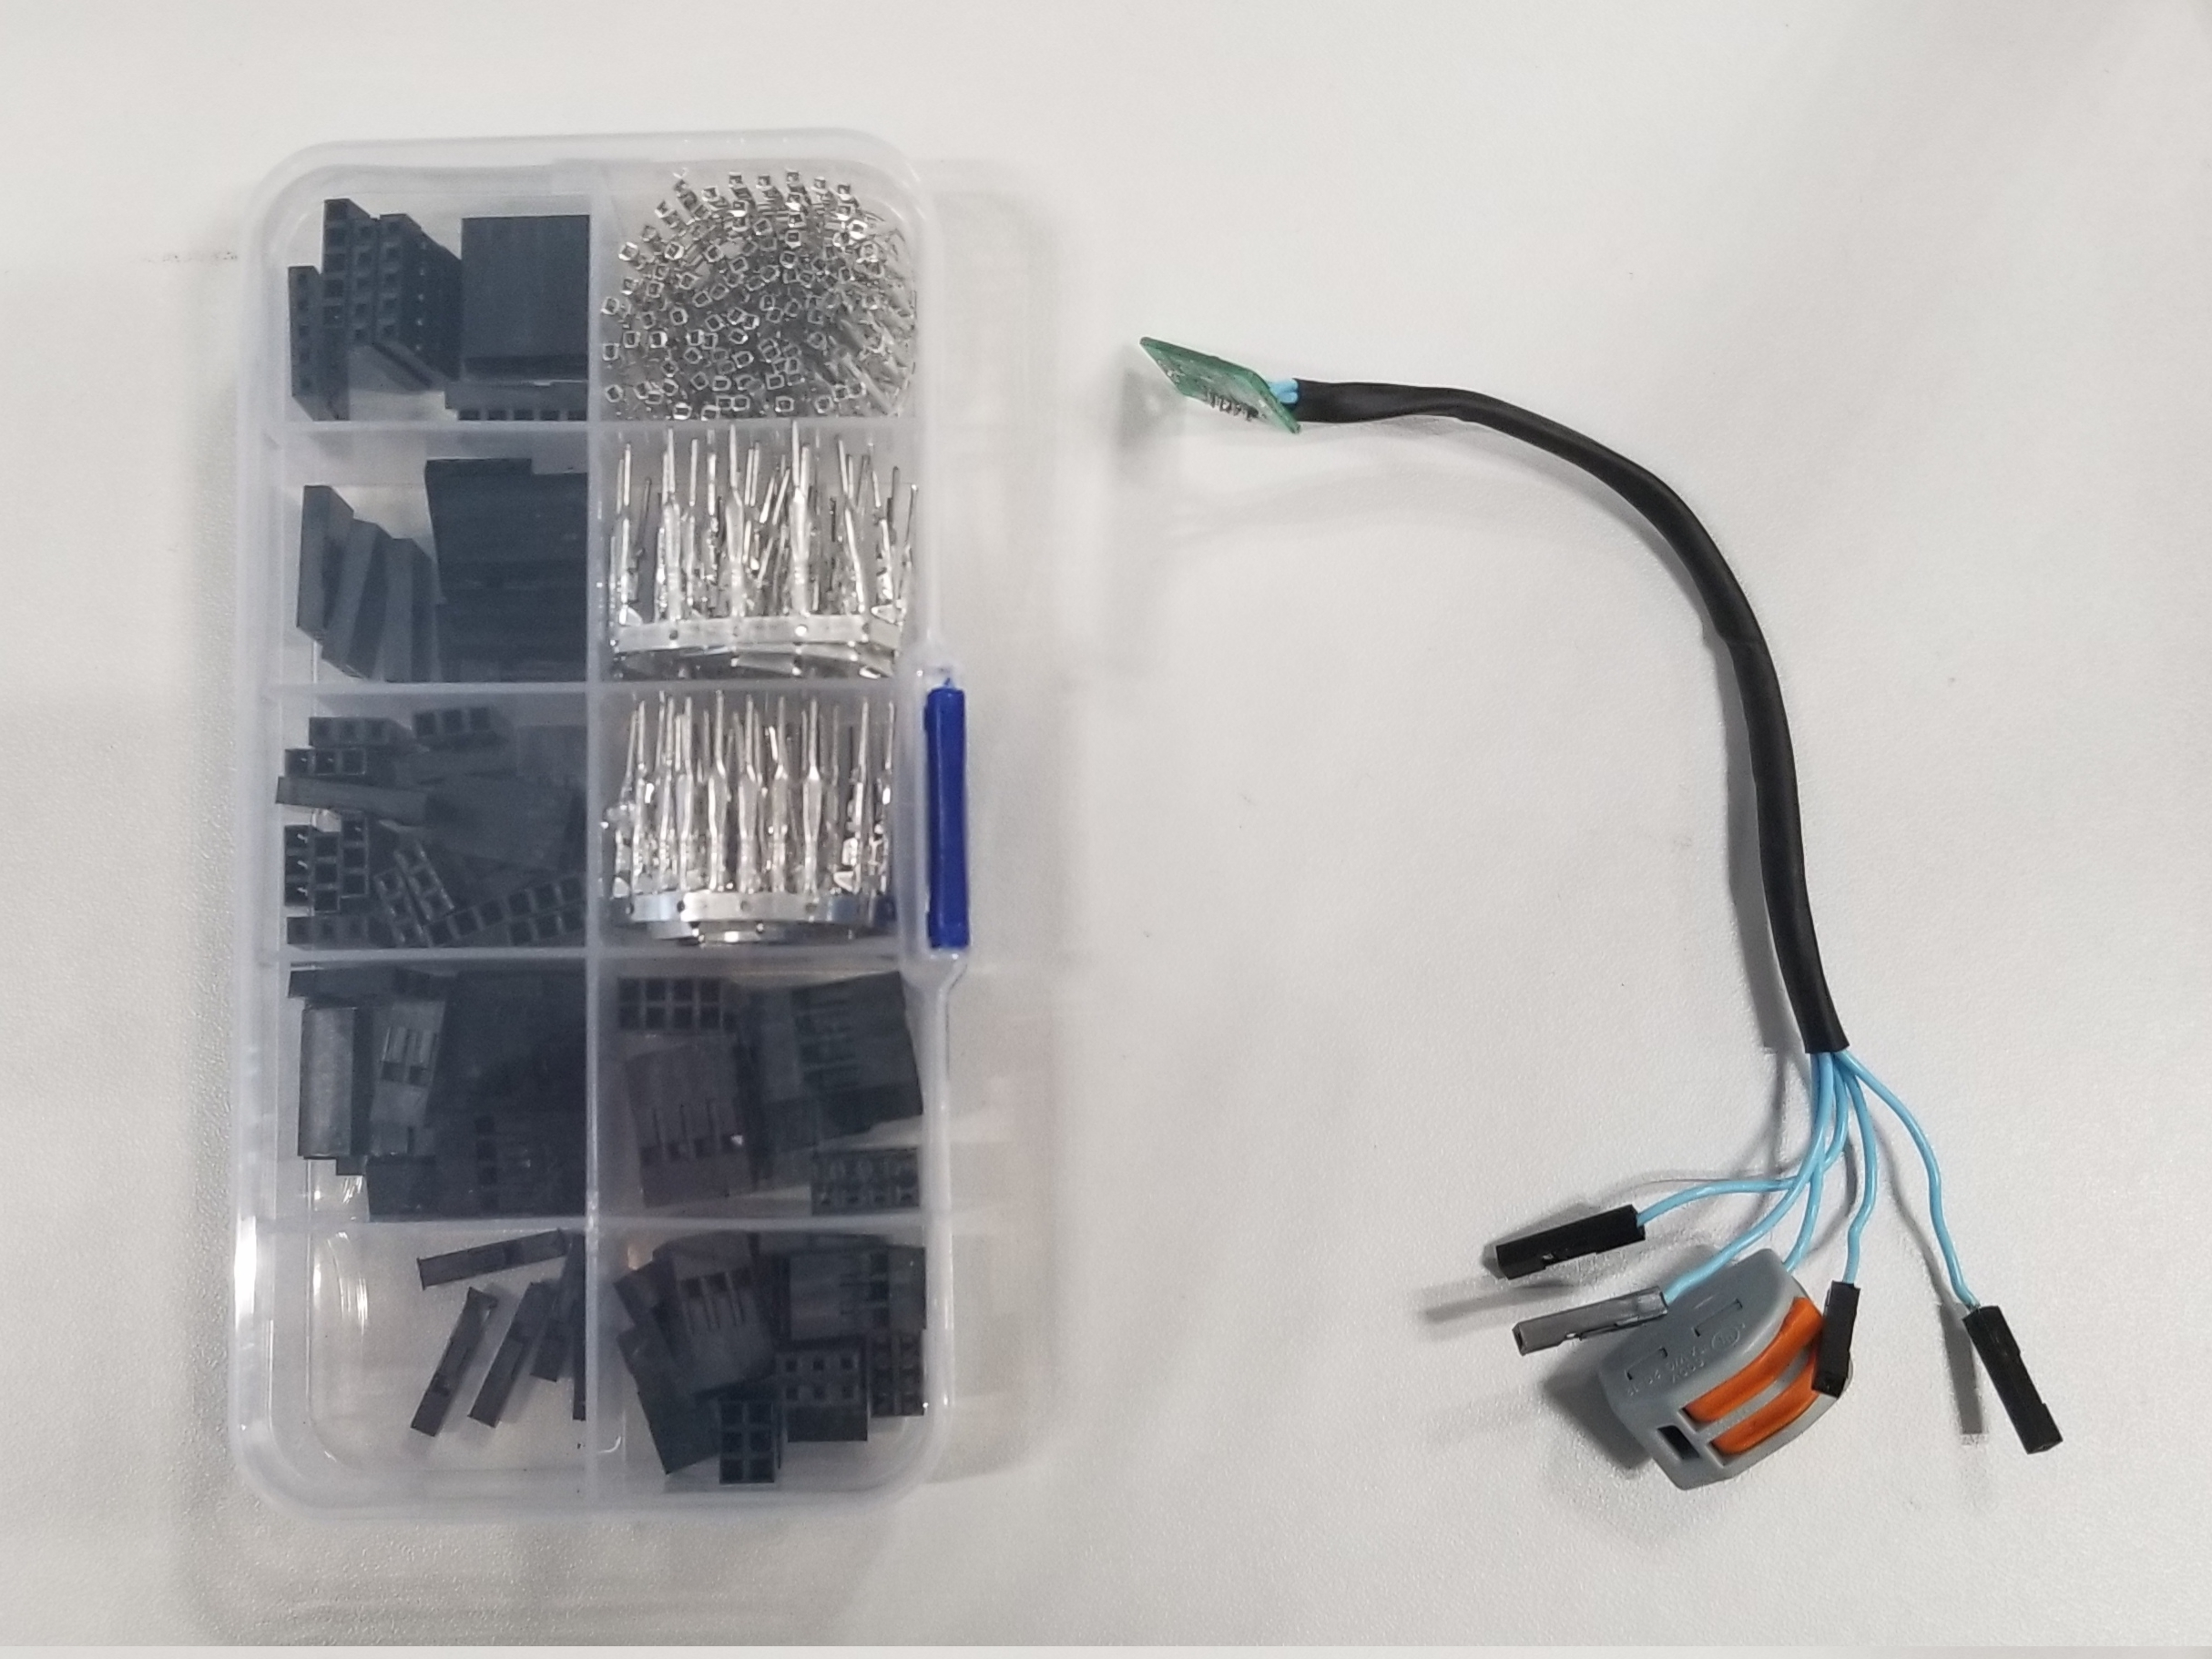
\includegraphics[scale=0.1]{../images/capteurQTR.jpg}

\subsection{Schéma EasyEDA}

\todo

% A detailed section of your code: approach, structure, etc.
\section{Logiciel}

\subsection{Architecture du programme}

Le développement des fonctions métiers du robot a été une étape importante dans la réalisation de notre robot.
En effet, nous avons dû développer des fonctions permettant de contrôler les différents composants de notre robot pour atteindre nos objectifs.

Pour garder le développement structuré, nous avons décidé de découper notre programme en plusieurs parties, généralement concrétisées par des classes.

Voici les différentes fonctions que nous avons développées :
\begin{itemize}
    \item Une couche d'abstraction matérielle.
    \item Journalisation des événements.
    \item Fonction permettant de contrôler les moteurs
    \item Fonction permettant de contrôler l'écran LCD
    \item Fonction permettant de contrôler le capteur de distance lidar
    \item Fonction permettant de contrôler le haut-parleur
    \item Fonction permettant de récupérer la position de la ligne
    \item Fonction permettant de contrôler le robot à distance à l'aide d'une interface de contrôle
    \item Fonction permettant de contrôler le robot automatiquement
\end{itemize}

\subsubsection{Couche d'abstraction matériel}

La couche d'abstraction matériel permettant de tester notre programme en intégration continue / machine locale ou sur le Raspberry Pi. 
Elle est basée sur des macros du préprocesseur C++.
Dans le cas d'une compilation sur le Raspberry Pi, les fonctions de la couche d'abstraction matériel sont remplacées par des fonctions permettant de contrôler les composants de notre robot.
Tandis que dans le cas d'une compilation en machine locale, les fonctions de la couche d'abstraction matérielle sont remplacées des messages de logs.
Ainsi, à la précompilation, le code est adapté à la plateforme cible (natif ou Raspberry Pi), et peut être testé sans avoir besoin d'un Raspberry Pi.

Les fichiers concernés sont \texttt{src/pin.h} et \texttt{src/pin.cpp}.

\subsubsection{Journalisation des événements}

Afin de pouvoir déboguer notre programme aisément, nous avons développé un système de journalisation des événements.
Ainsi, nous pouvons afficher des messages de logs sur la sortie standard de notre programme avec des couleurs différentes en fonction du niveau de criticité du message (erreur, avertissement, information, débogage et trace).
De plus, l'affichage peut être réglé aisément à la compilation en modifiant une macro (\texttt{LOG\_LEVEL}).

\subsubsection{Contrôle des moteurs}
Une classe Moteur a été créée afin de contrôler les moteurs de notre robot. Cette classe permet de contrôler la vitesse et la direction de nos moteurs.
Nous envoyons simplement des commandes au pont en H qui lui se charge de contrôler les moteurs.

\subsubsection*{Contrôle de l'écran LCD}
Une classe LCD a été créée afin de contrôler l'écran LCD de notre robot. Cette classe permet d'afficher des informations sur l'écran LCD de notre robot.
Nous envoyons des simples commandes au PCF8574T qui lui se charge de contrôler l'écran LCD.

\subsubsection*{Contrôle du capteur de distance lidar}
\todo
\subsubsection*{Contrôle du haut-parleur}

Pour envoyer des sons sur notre haut-parleur nous lançons simplement des commandes système qui permettent de jouer des sons sur notre Raspberry Pi qui sont ensuite envoyés sur notre haut-parleur.
\\
L'interface web est capable d'envoyer des commandes au robot pour jouer des sons.

\subsubsection*{Récupération de la position de la ligne}
Pour récupérer la position de la ligne nous utilisons une caméra. La caméra est en mode noir et blanc nous avons séparé l'image en 5 zones.
Nous faisons la moyenne des pixels de chaque zone et si cette moyenne est supérieure à un certain seuil alors nous considérons que la ligne est dans cette zone.



\subsubsection{Développement de l'interface de contrôle}
Nous avons décidé de nous tourner vers les technologies web pour développer l'interface de contrôle de notre robot. Celles-ci, par leur simplicité, nous ont permis d'avancer rapidement, et de nous concentrer plutôt sur le développement des fonctionnalités de notre robot. Les navigateurs offrent notamment un large support des manettes de jeux, et son intégration a donc été très simple.
Le robot fait tourner un serveur HTTP afin de recevoir les commandes du client. Internet étant accessible à travers le wifi de l'INSA, le robot peut donc être controlé à distance dans tout le périmètre de l'école. Disposant d'une caméra, il est possible de s'aider du flux vidéo pour contrôler le robot.
Néanmoins, le réseau de l'INSA nous faire subir quelques instabilités. Si la latence est très satisfaisante le plus souvent, il arrive au robot de perdre la connexion avec le client pendant quelques secondes. Ces problèmes de perte de contrôle du véhicule peuvent se révéler très problématiques. Nous désignons la DSI comme responsable d'éventuels accidents.
L'interface web nous a été très utile pour piloter le robot, mais aussi pour expérimenter avec différents paramètres, ainsi que pour visualiser l'état de certains capteurs. La plupart des paramètres et affichages des entrées ont été supprimées aujourd'hui.

\subsubsection*{Contrôle du robot à distance}
L'interface web envoie continuellement la position du joystick de la manette au robot. A partir de cette information, le robot calcule par une simple formule la vitesse de chaque moteur. Afin de réduire les problèmes de latence, l'interface web s'assure de ne pas envoyer les commandes plus rapidement que le robot ne les traite.

\subsubsection*{Contrôle automatique du robot}
Nous pouvons également changer le mode de fonctionnement de notre robot depuis l'interface web. Ce dernier peut ainsi entrer dans le mode "suiveur de ligne", se mettant ainsi à chercher et suivre automatiquement toute ligne noire présente en face de lui.

\section{Mécanique}
\subsection{Choix de la taille des roues}

Nous avons remarqué que le point fort des moteurs que nous possédons n'est pas leur vitesse de rotation, qui n'est pas spécialement rapide, mais plutôt leur couple.Autrement dit, l'utilisation de grandes roues ne ralentirait pas beaucoup la vitesse de rotation des moteurs mais augmenterait sensiblement la distance parcourue à chaque rotation. Nous avons donc opté pour de plus grandes roues. Malheureusement, la forme du point d'ancrage central des grandes roues ne correspondait pas aux moteurs, et celles-ci ne pouvaient donc pas être fixées directement. Nous avons donc modifié les roues de petite taille en y collant par dessus les roues de diamètre supérieur. Cette modification a entrainé d'autres changements sur notre robot comme l'utilisation d'une cale pour sur-élever notre roue folle ou encore la création d'une "pince à balle" plus grande que la norme. Cependant, nous avons tout de même gardé la possibilité d'utiliser à nouveaux des roues de petite taille car tous les ajouts que nous avons fait peuvent être facilement enlevés à l'aide d'un tournevis. En effet, il est parfois intéressant d'avancer moins rapidement, notamment dans le mode suiveur de ligne.

\subsection{Emplacement des roues et des capteurs}
Notre robot a connu beaucoup d'évolution tout au long du projet que cela soit au niveau du code ou de l'organisation des composants.

Initialement, nous avions placé les roues à "l'arrière du chassis" (à l'opposé de l'emplacement du capteur de distance) avec une roue folle vers l'avant. Cette disposition des roues convenait très bien à la conduite manuelle du robot car elle permettait une rotation rapide de l'avant. Cependant, nous avons également eu beaucoup de changements concernant le choix de nos capteurs de lignes (cf 3.1.1 et 5.1.3) et nous avons remplacé des capteurs placés sous le chassis par un autre placé tout à l'avant. La rotation rapide de notre robot est ainsi devenue un problème, perturbant les données captées par notre capteur à l'avant. De plus, la position reculée des roues faisait que le centre de pivot de notre robot était également reculé, et par conséquent, éloigné de notre capteur suiveur de ligne. C'est pour l'ensemble de ces raisons que nous avons finalement adapté la position de nos roues en les plaçant à l'avant, plus proche du capteur.

Ce changement nous a permis de meilleurs résultats sur l'algorithme du suiveur de ligne tout en gardant une maniabilité sensiblement inchangée pour le mode manuel.


% A section with detailing each member’s taks in the project + l'organisation interne
\chapter{Méthodologie}
    Pour réaliser ce projet, nous avons commencé par réaliser quelques recherches pour trouver des idées de comment nous pouvons atteindre nos objectifs.
    \\
    Après avoir récolté quelques idées, nous avons décidé de nous répartir les tâches en fonction des affinités de chacun avec les différentes parties du projet.
    \\
    Nous avons alors commencé à réaliser les différentes parties du projet en parallèle, en discutant régulièrement pour faire le point sur l'avancement du projet et afin de s'entraider si besoin mais surtout de comprendre les différentes parties du projet.
    \\
    Nous avons également utilisé un dépôt git pour pouvoir travailler sur les mêmes fichiers en même temps, et pour pouvoir revenir à une version antérieure si besoin ce qui nous aura été utile à plusieurs reprises.
    Une CI a également été mise en place afin de vérifier que le code compile et que les tests passent à chaque push sur le dépôt git pour éviter de casser le code sur le dépôt.
    \\
    À plusieurs reprises nous avons décidé de pivoter, pour cela nous avons dû parfois grandement modifié notre code et robot, nous pouvions donc créer une nouvelle branche afin de réaliser nos expérimentations sans risquer de casser le code fonctionnel.
    \\
    Pour travailler, la plupart du temps nous nous sommes réunis à l'INSA pendant les heures de TP, mais aussi souvent en dehors des heures de cours pour trvouer le temps de corriger les plus gros problèmes.
    \\




\chapter{Réalisation}
\lipsum[7-8]
\section{Difficultés rencontrées}
\subsection{Problèmes de son}
Au tout début du projet nous avons eu l'idée d'ajouter un haut-parleur à notre robot. L'idée était très simple : utiliser le port jack intégré à notre Raspeberry Pi pour émettre un son qui sera ensuite amplifié avant d'être émis par un haut-parleur. En fin de compte, cette fonctionnalité a été un vrai challenge à ajouter sur notre robot et c'est pour cete raison que nous y dédions une sous-partie du rapport. Nous détaillerons toutes les solutions essayées ainsi que la solution finalement retenue.
\\
La première solution censée apporter le son à notre robot a été le module d'amplification suivant : 386AMP from DFRobot
\\
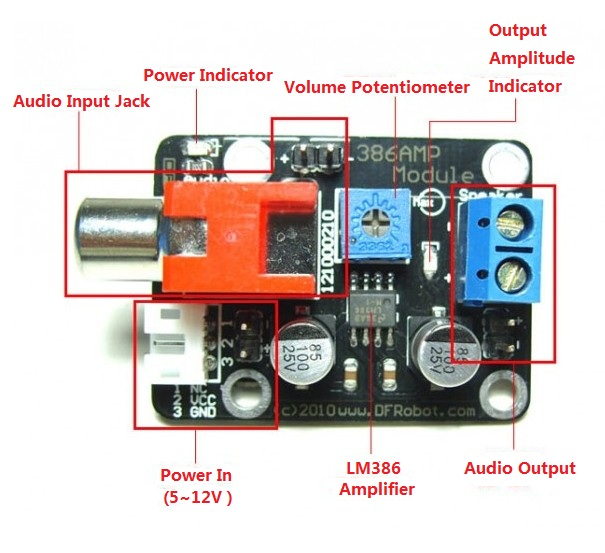
\includegraphics[scale=0.5]{386AMP.jpg}
\\
Cependant, il nous fallait un câble jack 3.5 vers RCA afin de pouvoir utiliser le module d'amplification sur lequel pouvait ensuite être aisément branché un haut-parleur. Étant donné que le laboratoire d'électronique ne possédait pas ce type de câble, nous avons fini par trouver le matériel nécessaire chez nous. Ainsi, nous avons pu faire les premiers tests du module avec nos téléphones. Ces derniers étant concluants, nous avons recherché les commandes nécessaires à la lecture d'un audio sur Raspeberry. Nous utilisons donc 3 fonctions systèmes
de la Raspeberry.
\begin{itemize}
    \item system("amixer -q set PCM,0 unmute"); permet de s'assurer que le son de la Raspeberry est actif
    \item system("mpg321 -q assets/" + filename + " \&"); permet de lancer, en processus d'arrière plan, l'audio désigné par la variable filename
    \item system("pkill -9 mpg321"); permet d'arrêtter le processus qui joue la musique en cours
\end{itemize}
Malheureusement, lors de notre premier test du module d'amplification sur la Raspeberry nous n'avons obtenu qu'un bip continu. Ce problème survient uniquement lorsque les autres fonctionnalités  de notre robot était en marche. Un autre groupe a été confronté à ce problème et malgré nos efforts communs et les nombreux cas similaires présents sur Internet nous n'avons jamais réussi à utiliser le module d'amplification.
\\
Les solutions que nous avons essayées sont pourtant nombreuses :
\begin{itemize}
    \item changement de configuration d'amixer (le logiciel gérant le son sur la Raspeberry)
    \item changement de matériel (module d'amplification et câble)
    \item changement de configuration du PWM (dont l'activation semble être à l'origine de notre problème)
\end{itemize}
En fin de compte, après l'échec de toutes ces solutions, c'est l'utilisation du MAX 98357A, un Amplifier/DAC (Digital Analog Converter), qui nous a permis de jouer des sons sur notre robot. Nous en avons donc conclu que le port jack de la Raspeberry était bien à l'origine de notre problème sans pour autant l'avoir résolu.

\subsection{Tentative d'algorithme suiveur de ligne PID}
Nous avons réalisé quelques recherches sur des algorithmes permettant de faire de l'asservissement et nous nous sommes rendus compte que l'algorithme le plus répendu est le PID Control.
L'objectif de cet algorithme est de faire en sorte que l'erreur entre la position actuelle du robot et la position désirée soit nulle. Pour cela, il faut calculer l'erreur, c'est à dire la différence entre la position actuelle et la position désirée, puis calculer la dérivée de cette erreur et enfin calculer l'intégrale de cette erreur.
Sur le papier, cet algorithme semble très simple à mettre en place. Cependant, nous avons rencontré de nombreuses difficultés lors de la mise en place de cet algorithme.
En effet, nous avons dû faire face à de nombreux problèmes de détection de ligne. En effet, nous avons essayé de faire fonctionner notre robot avec des capteurs QTR mais ces derniers ne fonctionnaient pas correctement. Nous avons donc essayé de faire fonctionner notre robot avec une caméra mais celles-ci n'avait pas un angle de vue assez large pour détecter la ligne suffisament loin pour le PID.

\subsection{Échec des capteurs QTR}
Nous avons essayé d'utiliser des capteurs QTR pour détecter la ligne. Cependant, nous avons rencontré de nombreux problèmes avec ces capteurs. En effet, nous n'avons rien trouvé sur internet qui nous permettait de les utiliser correctement avec un raspberry.
Nous avons donc développé notre propre code pour utiliser ces capteurs. Cependant, nous n'avons pas réussi à obtenir des résultats satisfaisants avec ces capteurs. En effet, ils détectaient trop de bruit et ne détectaient pas la ligne de manière fiable.
Nous ne savons pas si le problème venait de notre code ou des capteurs eux-mêmes mais nous avons finalement décidé de ne pas utiliser ces capteurs.
Nous nous sommes dit que le seul moyen de faire fonctionner notre robot correctement était d'utiliser une caméra. En effet, en observant une seule bande de pixel sur une image, nous pouvions détecter la ligne de manière fiable.


\section{Les capacités du robot}


\chapter{Conclusion}
% Partie dans laquelle on revient sur ces difficultés, on essaie de les raisonner
% (leur trouver une raison) et faire comme si le projet avait été une source incroyable d'apprentissage pour nous

Pour conclure ce rapport nous pouvons revenir sur tous ce que projet nous a apporté.

Sur le plan purement technique nous avons beaucoup appris ce robot étant notre première réalisation complexe en électronique. Nous avons pu mettre en pratique nos connaissances de cours, à l'instar de l'utilisation de Wiring Pi, du PWM, du protocole I2C et des différents composants utilisés durant les sessions en labo (TP), mais nous sommes également aller plus loin en apprenant de nouvelles choses. Nous pouvons notamment citer la gestion des threads, l'utilisation de nouveaux composants comme le DAC/Amplifier ou encore le LIDAR. Même nos échecs comme l'utlisation des capteurs QTR nous a permis dans en apprendre plus sur de nouveaux sujets. De plus, certains membres du groupe on pu découvrir de nouveaux outils pour la gestion de projet tel que PlatformIO ou easyEDA.

Le projet a aussi été une source d'apprentissage sur le plan organisationnel. La longueur du projet et le nombre important de fonctionnalités que nous voulions réaliser nous a obliger à fixer une organisation bien définie dès le début du projet. Cependant, il est important de remarquer que se sont les nombreuses difficultés que nous avons rencontrées au fur et à mesure des séances sont de bonnes expériences pour nos futurs projets. En effet, notre envie d'améliorer le plus possible notre robot nous a poussé à utiliser dès le départ des composants totalement nouveaux pour nous et de nous écarter des lignes toutes tracées du sujet. En raison de cette envie de faire toujours plus nous avons pris beaucoup de retards suite aux difficultés rencontrées, notamment sur les capteurs QTR dont l'abandon nous a forcé à changer successivement notre capteur de ligne, l'emplacement de nos roues et enfin notre algorithme suiveur de ligne sur les dernières séances.

Pour conclure, notre robot n'est peut-être pas le plus efficace mais le projet nous a apporté de nouvelles connaissances ainsi qu'une réelle expérience de gestion de projet qui nous permettra d'être bien meilleur sur nos prochaines réalisations.

% Bibliographie
\begin{thebibliography}{9}
    \bibitem{niControllerTheory}
    The {P}{I}{D} {C}ontroller \& {T}heory {E}xplained --- ni.com.
    \textit{National Instruments}.
    \url{https://www.ni.com/en/shop/labview/pid-theory-explained.html}.
    [Accessed 08-11-2023].

    \bibitem{PID Control}
    PID Controller Optimization for Low-cost Line
Follower Robots
    \\\texttt{https://arxiv.org/pdf/2111.04149.pdf}
\end{thebibliography}


\end{document}
